\documentclass{article}
\usepackage{graphicx} % Needed for including graphics.
\usepackage{amsmath}  % Needed for math features.

\title{Designing an Efficient Interpolation Method}
\author{ByeongKyu Park}
\date{\today}

\begin{document}
\maketitle

\section{The Idea}
This method introduces a straightforward and efficient approach for connecting data points with piecewise arcs. Unlike traditional interpolation techniques that might rely on complex computations and derivative information (e.g., $y'$ and $y''$ in cubic splines), this technique simplifies the process by adjusting the curvature of arcs based on relative slopes between segments. It's designed to efficiently handle large datasets, offering an $O(N)$ time complexity, which makes it significantly more efficient for quick analysis and visualization compared to methods like Lagrange or cubic splines that have higher computational demands.

\begin{figure}[htbp]
\centering
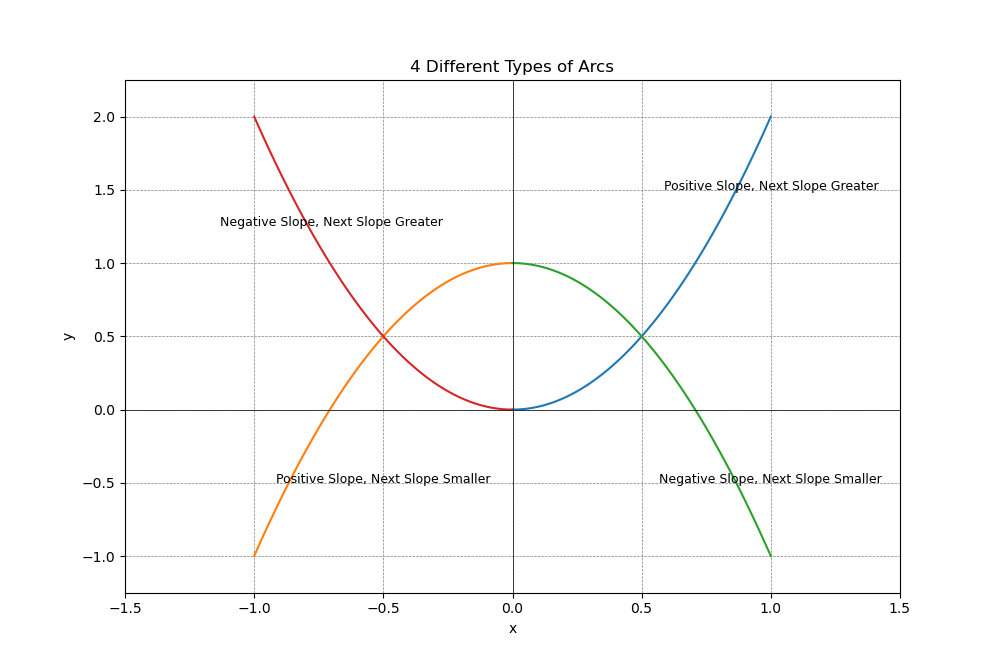
\includegraphics[width=0.8\textwidth]{4_arc_types.png}
\caption{Illustration of the 4 types of arcs used for interpolation.}
\end{figure}

\section{The Computation}
The computational framework involves:
\begin{enumerate}
    \item Calculating slopes between consecutive points to check the data trend.
    \item Assigning fixed curvatures(0.5) to arcs connecting these points, based on the trend analysis, which simplifies the visualization of data progression.
    \item Employing a sinusoidal function to model the curvature, facilitating a quick and intuitive representation of the dataset.
\end{enumerate}
This method doesn't necessitate derivative data, streamlining its application to large datasets where computational efficiency is of prime importance.

\section{The Results}
Below are the interpolated results for the given \(x, y\) values.

\begin{figure}[htbp]
\centering
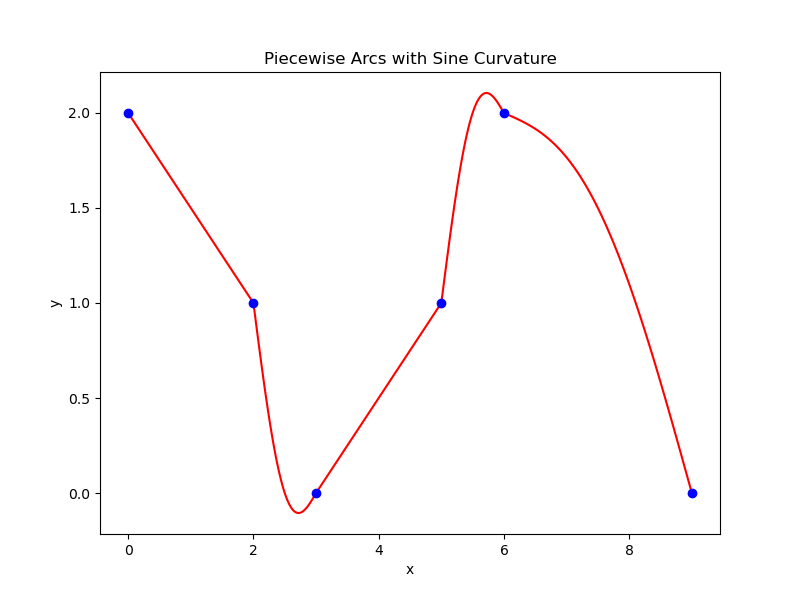
\includegraphics[width=0.8\textwidth]{test_case_1.png}
\caption{Interpolation on Dataset 1}
\end{figure}

\begin{figure}[htbp]
\centering
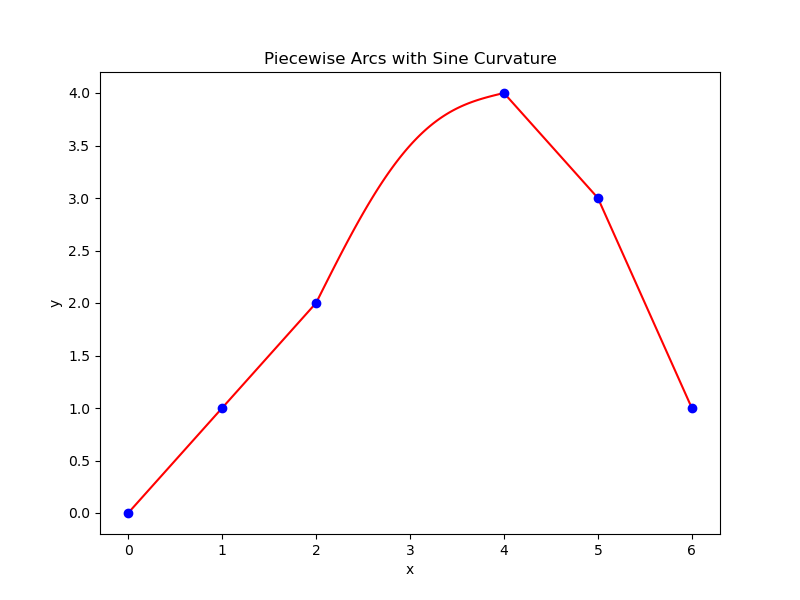
\includegraphics[width=0.8\textwidth]{test_case_2.png}
\caption{Interpolation on Dataset 2}
\end{figure}

\begin{figure}[htbp]
\centering
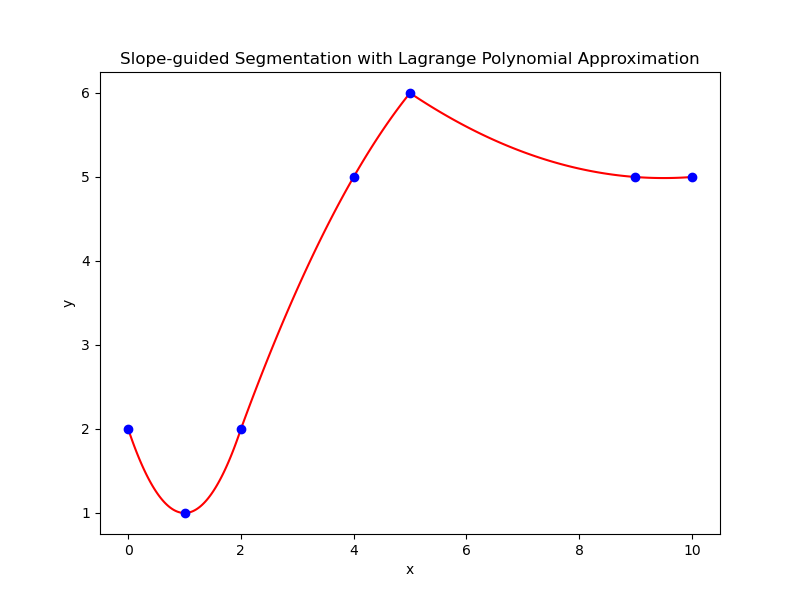
\includegraphics[width=0.8\textwidth]{test_case_3.png}
\caption{Interpolation on Dataset 3}
\end{figure}

\begin{figure}[htbp]
\centering
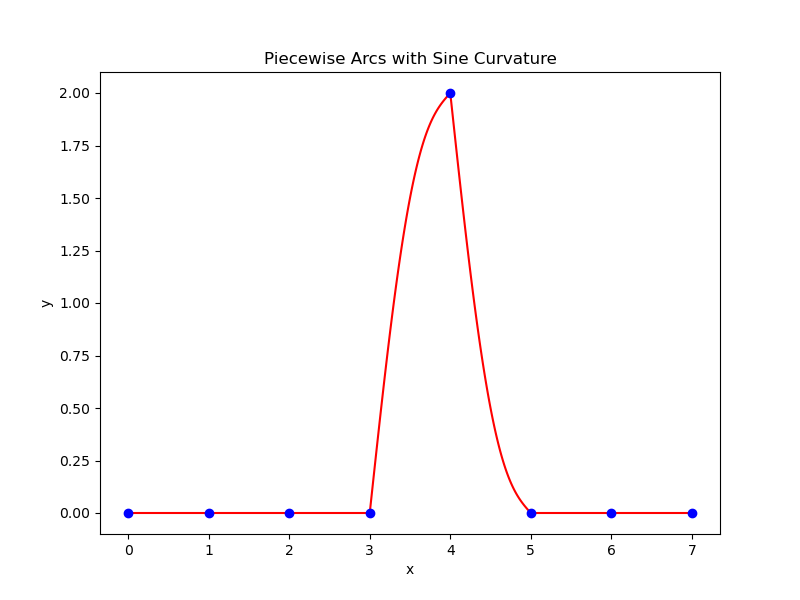
\includegraphics[width=0.8\textwidth]{test_case_4.png}
\caption{Interpolation on Dataset 4}
\end{figure}

\begin{figure}[htbp]
\centering
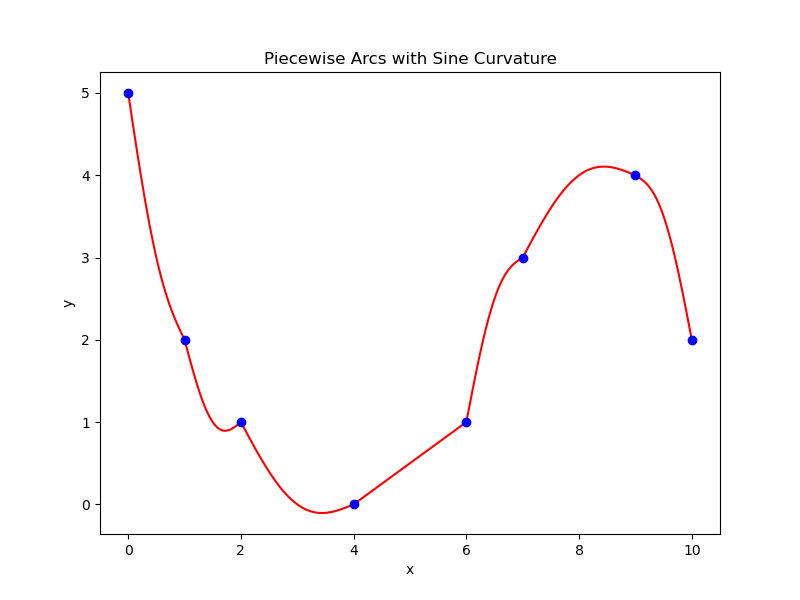
\includegraphics[width=0.8\textwidth]{test_case_5.png}
\caption{Interpolation on Dataset 5}
\end{figure}

\newpage
\section{Possible Issues}
While designed for simplicity and efficiency, this method encounters specific limitations:
\begin{enumerate}
    \item The adoption of fixed curvature values might not capture the nuanced variations within the data, potentially leading to a gap between the modeled and actual trends.
    \item Applying a uniform curvature approach could inadvertently introduce bends in data segments better represented by straight lines, distorting the true nature of the data's progression.
    \item This method may struggle with accurately representing datasets that exhibit sharp directional changes, where the fixed curvature cannot adequately adjust to the data's complexity.
\end{enumerate}

\section{Possible Extensions}
To address these limitations and broaden the method's applicability:
\begin{enumerate}
    \item A system that can change the curvature based on a closer look at how quickly the data's direction changes, making the curve fitting more precise.
	\item Analyzing the spacing of data points within segments can inform curve bending. This approach adjusts curvature based on point density, improving graph accuracy. When evaluating how points are spread out in each segment, the method could take into account both the distance between points and their distribution pattern. For segments where points are closely packed but vary widely in the \(y\) direction, it might introduce more curvature to accurately follow these fluctuations. Conversely, for longer segments where points are spread out but align more linearly, the method could opt for a subtler curve or even approach a straight line, reflecting the broader, more gradual trend. 
    \item Using different shapes, not just arcs, for connecting points could better match the actual data, especially for complex trends.
\end{enumerate}

\end{document}
